\section{Konzept}

Diese Sektion enthält eine Beschreibung des generellen Lösungsansatzes, der in
den einzelnen Phasen des Programmes verfolgt wird. Eine detaillierte Dokumentation
der konkreten Umsetzung befindet sich in Sektion \ref{module} - Modulbeschreibung.

Um eine hohe Erkennungsrate der Captchas zu erreichen und den Rechenaufwand
gering zu halten, haben wir uns dazu entschieden,
uns nicht ausschließlich auf die Funktion des neuronalen Netzes zu verlassen
und stattdessen im Programmablauf Vorbereitungsphasen zu integrieren, die die
Daten für das neuronale Netz aufbereiten. Durch diese Aufbereitung wollen wir
die Zahl der Inputneuronen gering halten und eventuelle Störsignale bereits im
Voraus entfernen. Aufgrund dieser Anforderungen haben wir uns bei der Umsetzung für Matlab entschieden, 
da es bereits passende Erweiterungen zur Aufbereitung von Bildern und zum
Erstellen von neuronalen Netzen speziell für die Mustererkennung bietet.


\subsection{Ablaufphasen des Programms}

Der Ablauf des Programms kann in folgende grobe Phasen unterteilt werden: 

\begin{itemize}

\item Trainingsphase

Erstellen des neuronalen Netzes.


\item Einlesen und Aufbereiten der Captchas

Liest die Captchas aus den Dateien ein und entfernt grobe Störsignale.


\item Segmentierung

Teilt die aufbereiteten Bilder in einzelne Zeichen und normalisiert die
Ausrichtung.


\item Datenaggregation

Zusammenfassen von verwandten Datensätzen, um die Anzahl der Eingaben zu reduzieren.


\item Klassifizierung

Erkennen der Zeichen durch das neuronale Netz

\end{itemize}


\subsubsection{Trainingsphase}

Die Trainingsphase ist die Phase, in der ein neuronales Netz zum Erkennen der
Zeichen erstellt wird. Sie soll nur dann aufgerufen werden, wenn
nicht bereits ein vorbereitetes Netz existiert. In der Trainingsphase werden
vorbereitete Captchas zusammen mit der Lösung eingelesen und analog zu den
normalen Bildern aufbereitet. Die einzelnen Zeichen werden zusammen mit dem
Ergebnis zum Trainieren des Neuronalen Netzes verwendet. Die Trainingsphase
soll so lange andauern, bis sich zwischen den einzelnen Trainingsphasen keine
relevante Verbesserung ergibt.

\subsubsection{Einlesen und Aufbereiten der Captchas}

\begin{wrapfigure}[6]{r}{5cm}
  \begin{center}
  \vspace{-48pt}
    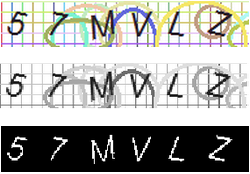
\includegraphics[width=4cm]{res/Aufbereitung.png}
  \end{center}
  \caption{Aufbereitung eines Captchas}
\end{wrapfigure}

In diesem Schritt werden alle Bilder aus einem Eingabeverzeichnis eingelesen und
aufbereitet. Die Aufbereitung versucht alle Pixel, die nicht zum eigentlichen
Text gehören, herauszufiltern. Zudem werden Farben durch binäre Werte ersetzt,
die entweder Schwarz oder Weiß darstellen. Hierbei wird anhand eines
Schwellwertes unterschieden, ab wann ein Graustufenwert als Schwarz oder als
Weiß gilt. Eine genauere Beschreibung der Aufarbeitung der Bilder befindet sich
in Kapitel \ref{images} - Aufbereitung von Bildern mit der Matlab-Image-Toolbox.


\subsubsection{Segmentierung}
\label{segment}

  \begin{wrapfigure}[6]{R}[0pt]{6cm}
  \vspace{-35pt}
  \begin{center}
    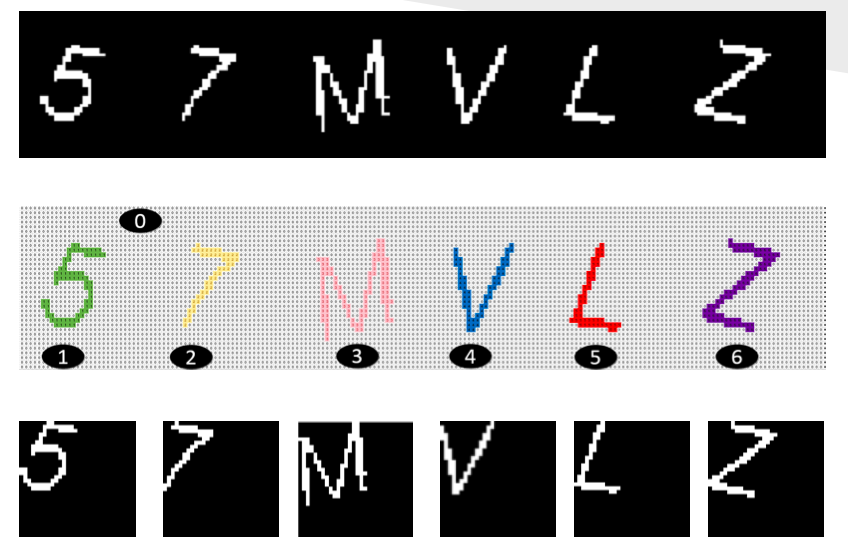
\includegraphics[width=5cm]{res/Segmentierung.png}
  \end{center}
  \vspace{-5pt}
  \caption{Segmentierung}
  \vspace{-10pt}
\end{wrapfigure}


Bei der Segmentierung wird versucht die Zeichen des Wortes in einzelne Segmente
zu unterteilen. Da das neuronale Netz eine konstante Menge an Eingabewerten
benötigt, wird zudem die Auflösung der Segmente auf eine einheitliche Größe
festgelegt. Alle Zeichen werden auf die gleiche Art ausgerichtet um
Verschiebungen auszugleichen.

\subsubsection{Datenaggregation}

\begin{wrapfigure}[15]{R}[0pt]{7cm}
  \begin{center}
    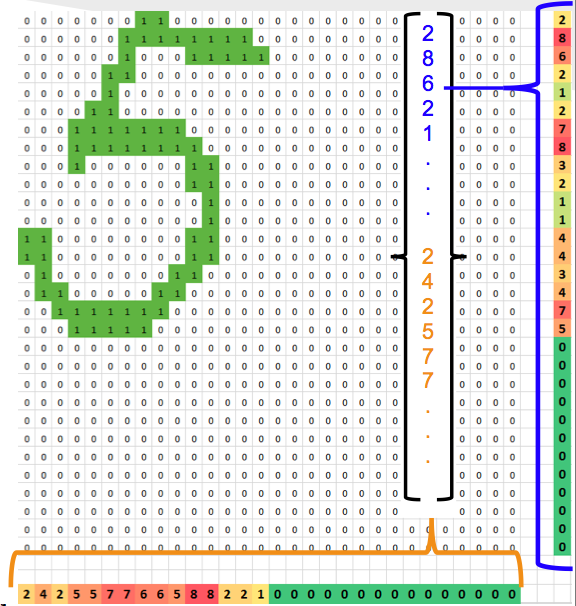
\includegraphics[width=6cm]{res/Aggregation.png}
  \end{center}
  \vspace{-5pt}
  \caption{Aggregation der Spalten/Zeilen}
  \vspace{-10pt}
\end{wrapfigure}


Bei der Datenaggregation wird versucht die Menge an Eingabewerten zu reduzieren,
ohne dabei viel Genauigkeit zu verlieren. Dies wird erreicht indem 
die Summen aller Schwarzen Pixel pro Zeile und Spalte gebildet werden. Ohne diese Aggregation, also bei direkter Eingabe aller Pixel in das
neuronale Netz, wäre die Laufzeit des Lernvorgangs und der Mustererkennung zu
hoch, um das Programm sinnvoll verwenden zu können.
\subsubsection{Klassifizierung}

Die Klassifizierung benutzt das neuronale Netz, um die eigentliche
Mustererkennung durchzuführen und so die einzelnen Buchstaben zu
erkennen. Jede Summe aus der Datenaggregation wird als einzelner Eingabewert
für das Netz verwendet. Diese Werte sollen in Matlab in Form eines Vektors zu
einem Set aus Eingabewerten für ein einzelnes Zeichen zusammengefasst werden.

\section{Struktur des neuronalen Netzes}

Um festzustellen wie viele Hidden-Neuronen das Netz braucht, wurde die
Leistungsfähigkeit des Netzes bei verschiedenen Mengen an Neuronen getestet.
Um die Leistungsfähigkeit der Netze festzustellen, wurde der Prozentsatz der richtig
erkannten Captchas ausgewertet und mit den anderen Netzen verglichen. 

Für jede Messung wurde automatisiert ein neues neuronales Netz mit der aktuellen
Anzahl der Hidden-Neuronen erstellt und dessen Leistungsfähigkeit gemessen.
Die Ergebnisse der Messung sind in folgender Grafik dargestellt:

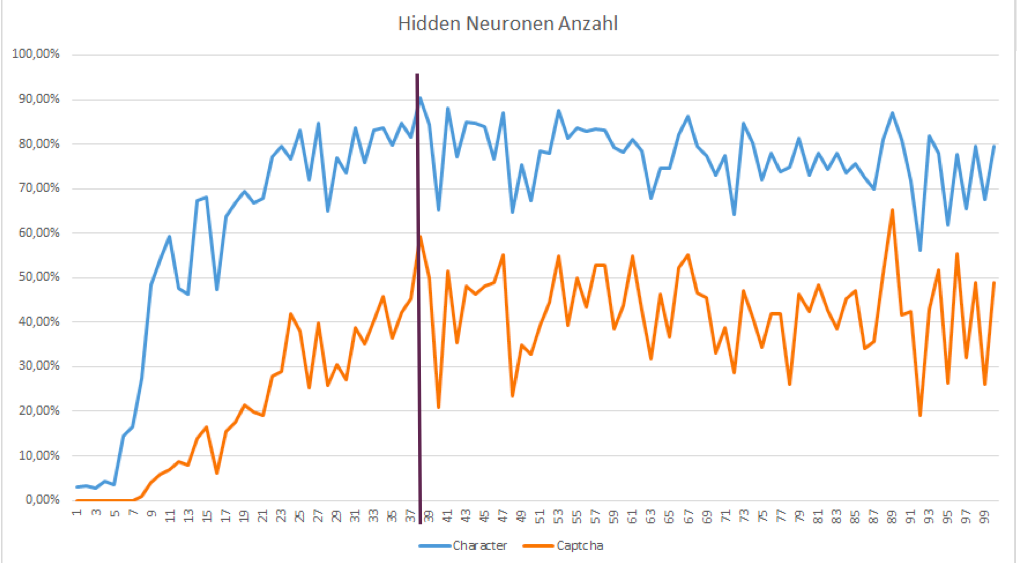
\includegraphics[width=14cm]{res/performance.png}

Da der Anstieg der Leistungsfähigkeit ab etwa $38$ Hidden-Neuronen aufhört,
legen wir die Anzahl dieser auf $38$ fest.

\subsection{Matlab - Die Klasse ``Patternnet''}

In der Matlab-Toolbox für neuronale Netze existiert bereits ein vorgefertigtes
neuronales Netz für die Mustererkennung. Diese Klasse nennt sich ``Patternnet''
und erbt von der Basisklasse ``nnet''. Die Klasse erstellt ein Feedforward-Netz
mit der Lernfunktion ``trainscg'', die die konjugierte Gradientenmethode zum
Lösen der Gleichungssysteme, die die neuen Gewichtungen bestimmen, verwendet.


  \begin{center}
    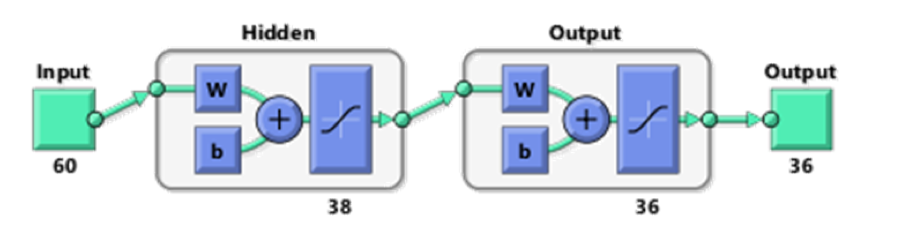
\includegraphics[width=12cm]{res/PatternNet-Aufbau.png}
  \end{center}


\subsection{Transferfunktion}
 Als Transferfunktion wird ein Sigmoid mit der folgenden Gleichung verwendet:

\begin{wrapfigure}[10]{R}[0pt]{7cm}
  \begin{center}
    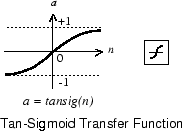
\includegraphics[width=6cm]{res/tansig.png}
  \end{center}
\end{wrapfigure}

\begin{equation}
n = tansig(n) =  \frac{2}{(1 + e^{-2*n})} - 1
\end{equation}

Der Wert von $n$ berechnet sich aus den aufsummierten, gewichteten
Eingsangswerten:

\begin{equation}
  n = w_1 * i_1 + w_2 * i_2 + \ldots  + w_j * i_j
\end{equation}

Das Sigmoid bewirkt, dass sich die Ausgabewerte eines Neurons ausschließlich
im Bereich $[-1,1]$ befinden. Zudem ist die Funktion einfach ableitbar, was
hilfreich beim aktualisieren der Gewichtungen während des Lernvorgangs ist.

\subsubsection{Lernfunktion}

In jeder Runde des Lernvorgangs müssen die Gewichte des Netzes so verändert werden,
dass sie möglichst nah am gewünschten Ausgangswert liegen. Hierfür ist es
notwendig ein Gleichungssystem zu lösen, um den optimalen Wert zu finden. Die Lernfunktion
des ``Patternnet'' verwendet hierfür die konjugierte Gradientenmethode, die ein
numerisches, iteratives Verfahren zum Lösen des Gleichungssystems darstellt.


\section{Aufbereitung von Bildern mit der Matlab-Image-Toolbox}
\label{images}

Für die Aufbereitung der Captchas werden Funktionen aus der Matlab
Image-Toolbox verwendet. Die Wichtigste ist hierbei die Funktion $regionprops$,
die dazu in der Lage ist, auf einem Bild Regionen mit bestimmten Eigenschaften
zu markieren. So ist es beispielsweise möglich, Regionen die sich in ihren Farbwerten 
nicht stärker als ein bestimmter Grenzwert unterscheiden, zu markieren.
Mithilfe dieser Technik werden auf dem Captcha zusammenhängende Buchstaben 
gefunden. Bei der Segmentierung, die in Sektion \ref{segment} beschrieben wird,
ist es essenziell diese Regionen zu kennen, um zu vermeiden dass die Zeichen an
der falschen Stelle zerteilt werden.

% \subsection{Darstellung von Bildern in Matlab}
% Bilder werden in Matlab generell wie Matritzen behandelt. Je nach Farbtiefe der
% Bilderm enthält jeder Wert entweder einen RGB- oder Graustufenwert. 
